\section*{Question 2}
\fakesection{2}

This problem goes in reverse to Question 1 by upsampling the downsampled signal back to the original sampling rate. We compare separately upsampling then filtering the signal versus applying a polyphase interpolator.

Beginning with the signal of Figure \ref{fig:q1_polydecimate}, we zero-pack the signal with $L-1=79$ zeros between each element to return to the original sampling rate of 40 kHz.

\begin{figure}[ht]
    \centering
    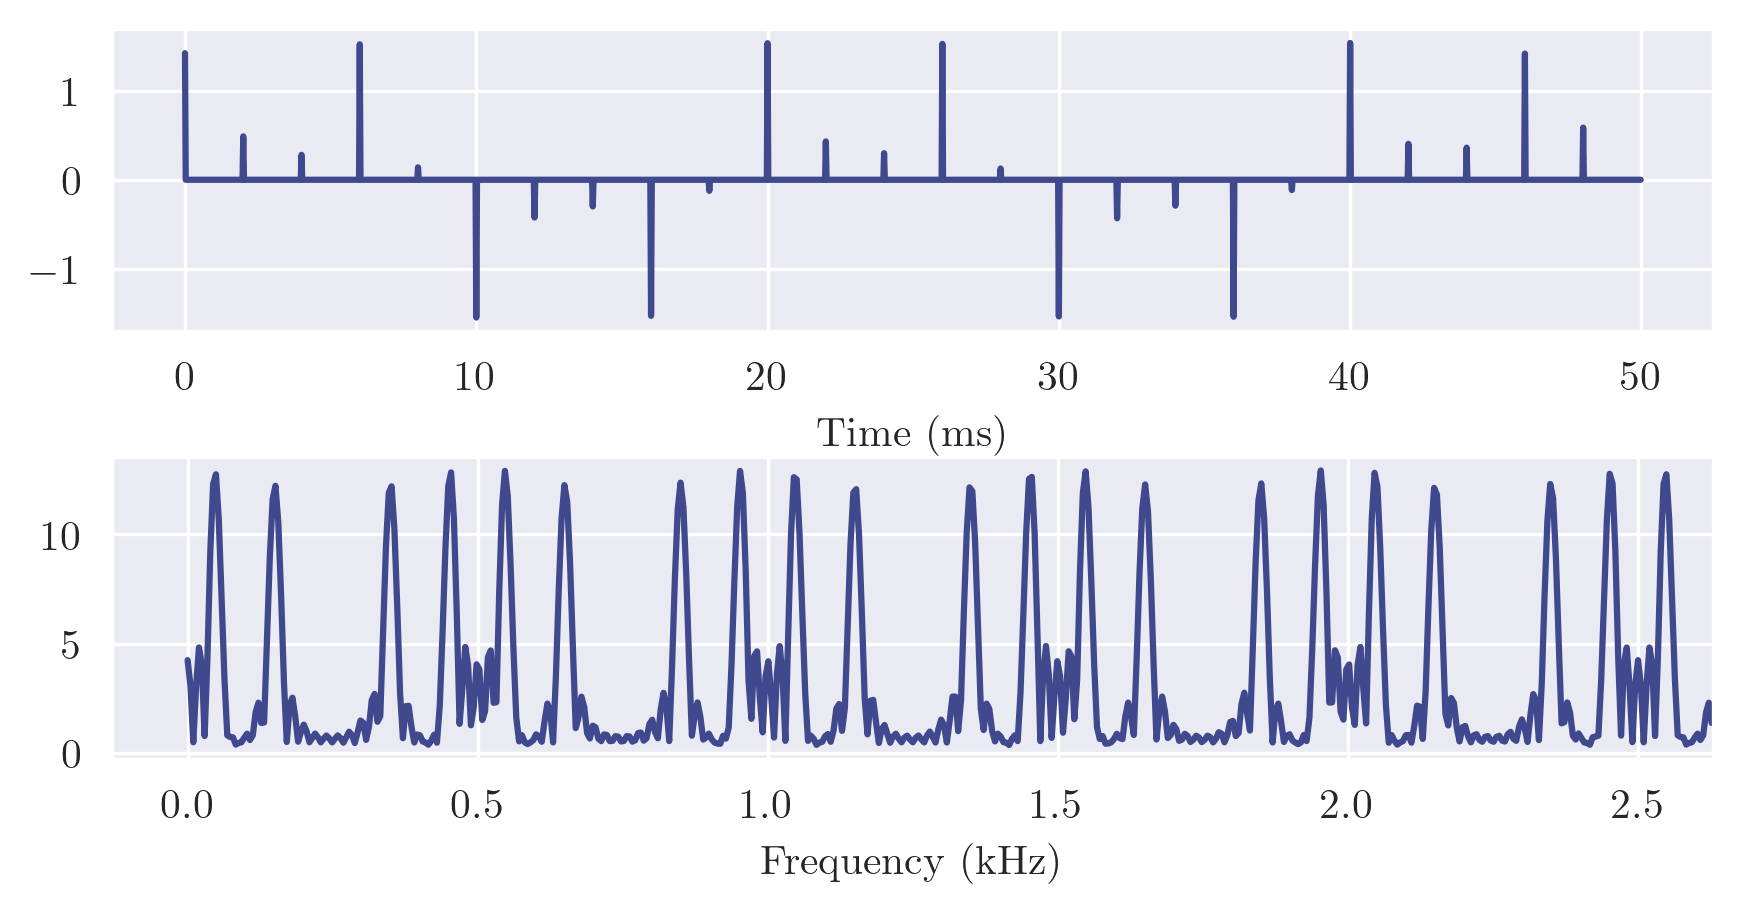
\includegraphics[width=0.8\textwidth]{images/q2_zpack.png}
    \caption{Zero-packed signal upsampled by $L$=80 back to 40 kHz}
    \label{fig:q2_zpack}
\end{figure}

As always, the zero-packing produces many undesirable copies of the frequency spectrum, which we remove by applying the same Kaiser-windowed filter of Question 1.

\begin{figure}[ht]
    \centering
    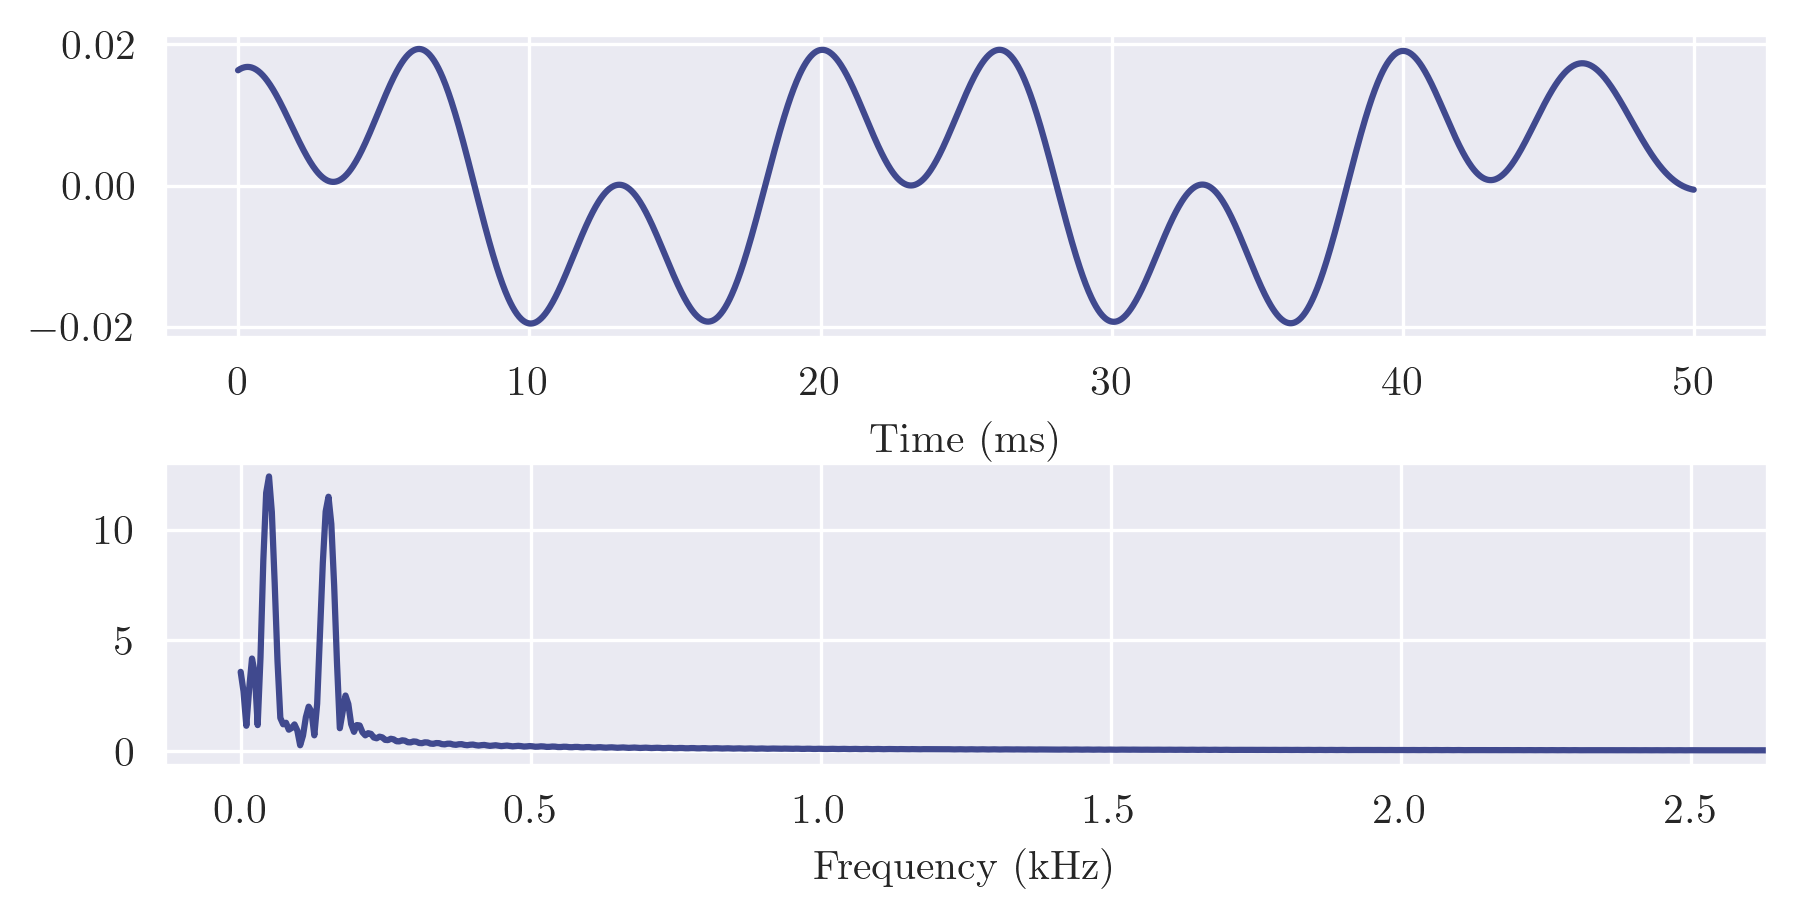
\includegraphics[width=0.8\textwidth]{images/q2_usamp.png}
    \caption{Zero-packed signal filtered to contain only 50 and 150 Hz tones}
\end{figure}

We now investigate repeating the upsampling and filtering using a polyphase interpolator. As before, we zero-pad the Kaiser-windowed LPF coefficients to a multiple of $L$, then reshape it into a column-major matrix with $L$ rows. We convolve each row of filter coefficients with the entire input signal and store the resulting $L$ sequences in a matrix. Finally, we construct the output signal by flattening the matrix back into a vector in column-major order.

\newpage

\begin{figure}[ht]
    \centering
    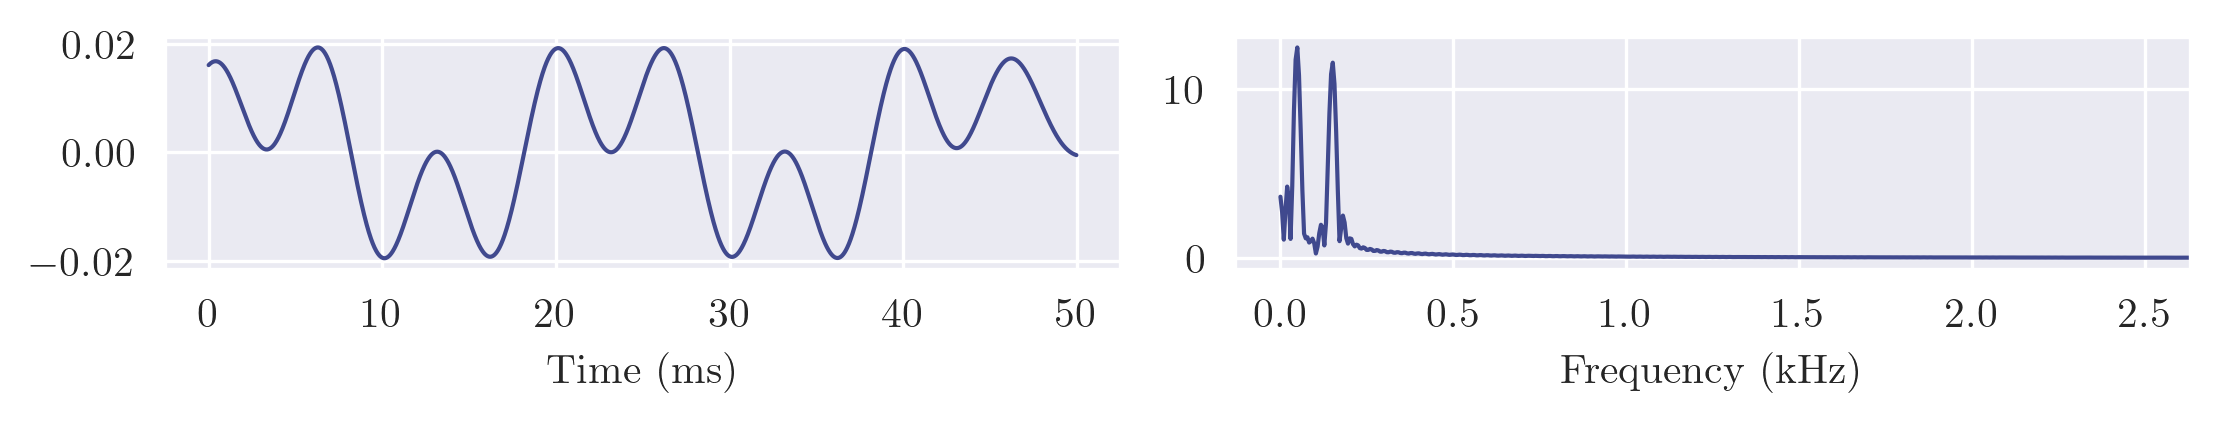
\includegraphics[width=0.8\textwidth]{images/q2_polyinterpolate.png}
    \caption{Polyphase interpolator applied to downsampled signal of Question 1}
    \label{fig:q2_polyinterpolate}
\end{figure}

Observe that the polyphase interpolator produces the same result as separately upsampling the filtering, and also reproduces the original filtered signal of Figure \ref{fig:q1_filt}. However, per the second noble identity, the polyphase interpolator requires a factor of $L$ less computations to achieve the same result, compared to upsampling then filtering. By a similar logic to the first noble identity from Question 1, by upsampling before filtering, $L-1$ elements of the upsampled signal are zero, representing meaningless computations during filtering. By filtering before upsampling, the polyphase interpolator achieves a theoretical $L$-fold performance gain.

As in Question 1, we can test this by timing repeated trials of either method as a proxy for the number of computations. Using 10,000 trials, we find the following average times:
\begin{itemize}
    \item Upsample then filter: 1.529 ms
    \item Polyphase interpolator: 0.801 ms
\end{itemize}
Following from the discussion for Question 1, while the polyphase filter is undoubtedly faster, we find in practice a much smaller performance benefit. This is an implementation specific caveat, and exhaustive investigation and optimisation is out of the scope of this problem.
